\documentclass[12pt,letterpaper,noanswers]{exam}
\usepackage[usenames,dvipsnames,svgnames,table]{xcolor}
\usepackage[margin=0.9in]{geometry}
\renewcommand{\familydefault}{\sfdefault}
\usepackage{multicol}
\usepackage{wrapfig}
\pagestyle{head}
\definecolor{c03}{HTML}{FFDDDD}
\header{AM 22b Class 17}{}{Mar 10: Monte Carlo + parameterization}
\runningheadrule
\headrule
\usepackage{graphicx} % more modern
\usepackage{amsmath} 
\usepackage{amssymb} 
\usepackage{hyperref}
\usepackage{tcolorbox}

\usepackage[numbered,autolinebreaks,useliterate]{mcode}

\newcommand{\mb}[1]{\underline{#1}}

\begin{document}
 \pdfpageheight 11in 
  \pdfpagewidth 8.5in




% I need to review the torus trajectories...

\begin{itemize}
% \item There is a pre-class assignment (20 minutes of videos + a few WeBWorK exercises) due at 10am this Monday.  It is available on Canvas.
\itemsep0em
    \item Problem set 05 is due on Thursday Mar 11th at 6pm.
  %  \item The Quiz 01 follow up assignment is due on Wednesday Mar 4th at midnight.
    \item The next skill check will be for C16, C17, C18 on Monday Mar 15th.
    \item My Wednesday OH is short today: 4:30-5pm on Wednesday.  The extra time will be an OH on Thursday from 2:30-3pm this week.
    \item There will be a pre-class assignment for Monday Mar 15th.
\end{itemize}

\hrule
\vspace{0.2cm}

% partial derivatives, gradient
% local linearity, differential, directional deriv
% 2nd order partials + equations with partials

\noindent\textbf{Big picture}

We are finishing our introduction to integration for functions of multiple variables with numerical approximation of integrals.  Next, we will build two tools (parameterized curves and vector fields) before studying integrals along curves.  These curves will not be restricted to straight lines along an axis, so we will need to generalize our single-variable calculus idea of an integral to work with these. 

\vspace{0.2cm}
\hrule
\vspace{0.2cm}



\noindent\textbf{Skill Check C17 Practice}
\begin{questions}
\question (parameterization of a circle). Provide a parameterization for a circle of radius $2$, centered at $(1,5)$, and traversed counterclockwise.  Traverse the circle once.  Choose a parameterization so that the traversal takes time $20$.

\end{questions}


\vspace{0.2cm}
\hrule
\vspace{0.2cm}

\noindent\textbf{Skill Check C17 Solution}

One way to parameterize a circle is by using a variation on polar coordinates.  The circle is of radius $2$, so set $x(t) = 2\cos t$ and $y(t) = 2\sin t$.  This circle is centered at $(0,0)$ and it takes time $2\pi$ to traverse it.  The traversal direction (as $t$ increases) is counterclockwise.

Now make some adjustments: first shift the center of the circle.  Let $x(t) = 1+2\cos t$ and $y(t) = 5 + 2\sin t$.  The center of the circle has been shifted to $(1,5)$.

Next adjust the traversal time.  We want the input to $\sin$ and $\cos$ to be $2\pi$ when $t = 20$.  Write $x(t) = 1+2\cos kt$ and $y(t) = 5+2\cos kt$.  At time $t=20$ we want $kt = 2\pi$.  So $20k = 2\pi$ and $k = 2\pi/20 = \pi/10$.

Our parameterization of the circle is

$x(t) = 1+2\cos(\pi t/10)$ and $y(t)=5+2\sin(\pi t/10)$, $0\leq t\leq 20$.

Notice that I have included the time range in my answer (so that we traverse the circle exactly once).

\vspace{0.2cm}
\hrule
\vspace{0.2cm}

\noindent\textbf{Teams}

You will work with this team on the in-class problems today.
\begin{multicols}{2}
1.  student names

\end{multicols}

%\vspace{0.2cm}
\hrule
\vspace{0.2cm}


\noindent\textbf{Monte Carlo integration: other domains} (not in text)
\begin{tcolorbox}
To use \textbf{Monte Carlo integration} over a region, $R$ that is not the unit box:
\begin{itemize}
\itemsep0em
    \item Create a rectangular box that encloses the region, $R$ and has area $A_{box}$.
    \item Define the function piecewise: it will be $0$ everywhere that is outside $R$.  It will be $f(\underline{x})$ in the region $R$.
    \item To use Monte Carlo integration on the rectangular box, generate $N$ random points within the rectangular box.  Use an even weight quadrature, where the weight assigned to the function evaluated at each point is $A_{box}/N$.  Think of each random point as representing $1/N$th of the box, so the associated area is $A_{box}/N$.
    \begin{lstlisting}
% Example
fc = @(x,y) x.^2 + y.^2;
npoints = 10000;
xyvals = rand(npoints,2);
xyvals(:,1) = xyvals(:,1)*5;
xyvals(:,2) = xyvals(:,2)*7;
integral = sum(fc(xyvals(:,1),xyvals(:,2)))*5*7/npoints;
\end{lstlisting}
\end{itemize}

\textbf{Pseudocode} is a description of the steps in a computer program, where the instructions may be written in human language, rather than in the syntax of a programming language.
\end{tcolorbox}

    \noindent\textbf{Example} (A non-unit interval in Matlab)
    
    \texttt{5*rand(1)} generates a random number uniformly spaced between $0$ and $5$.  \texttt{4*rand(1)+1} generates a random number uniformly spaced between $1$ and $5$.
    
    Write pseudocode to generate a pair of random numbers with one between $-1$ and $1$ and the second between $2$ and $4$.
    \vspace{1in}
    
    \eject

\noindent\textbf{Example: Approximating $\pi$}

Let $f(x,y) = 4$.  Let $R$ be the region in the first quadrant where $x^2+y^2\leq 1$.  $\int_R f(x,y) dA = \int_0^{\pi/2}\int_0^1 4r\ dr\ d\theta = \pi$.

Approximate this numerically to find an estimate for $\pi$.
\begin{lstlisting}   
npoints = 100000;
xyvals = rand(npoints,2);
indomain = (xyvals(:,1).^2+xyvals(:,2).^2)<1; %set to 1 if in domain; 0 if not
sum(4*indomain)/npoints
\end{lstlisting}

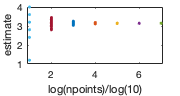
\includegraphics{img/C15Mpi.png}
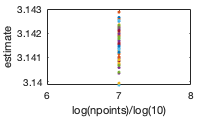
\includegraphics{img/C15MCpi7.png}
\vspace{0.1cm}

\noindent\textbf{Example: circular region}

Approximate the integral of a function that is not uniform: let $f(x,y) = xy$.  Let $R$ be the region in the first quadrant where $x^2+y^2\leq 1$.

\begin{lstlisting}
fc = @(x,y) x.*y;
npoints = 100000;
xyvals = rand(npoints,2);
indomain = (xyvals(:,1).^2+xyvals(:,2).^2)<1; %set to 1 if in domain; 0 if not
sum(fc(xyvals(:,1),xyvals(:,2)).*indomain)/npoints
%% Analytically:
int(int(fc(x,y),x,0,sqrt(1-y.^2)),y,[0,1])
\end{lstlisting}

\vspace{1in}

% \noindent\textbf{Example}

% %\begin{tabular}{p{12cm} c }
% Provide pseudocode for using Monte-Carlo integration to approximate the area, $\int_R dA$, where $R$ is the crescent shape shown. %&

% 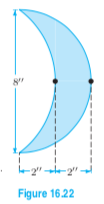
\includegraphics[scale=0.65]{img/C16crescent.png}
% %\end{tabular}

\eject

\vspace{0.2cm}
\hrule
\vspace{0.2cm}

\noindent\textbf{Parameterized curves} \S 17.1 

\begin{tcolorbox}
\begin{itemize}
\itemsep0em
    \item A function $f: \mathbb{R} \rightarrow \mathbb{R}^2$ is a \textbf{vector-valued function} because there are multiple outputs associated with each input.  
    
    The output of the function can be interpreted in two different ways: (a) as a mapping assigning a vector in $2$-space to each point along an axis, or (b) as a mapping assigning a point in $2$-space to each value of a parameterizing variable (often thought of as time).
    \item The set of equations 
\[x = f(t), \quad y = g(t), \quad z = h(t), \quad a\leq t \leq b\]
map a value of $t\in [a,b]$ to a point $(x,y,z)$ in 3-space.  For $f,g,h$ continuous functions, the set of points \[\{(x,y,z): x= f(t), y=g(t), z= h(t), a\leq t \leq b\}\] is a \textbf{parameterized curve} in 3-space with parameter $t$.
\item Even when the output is being interpreted as a position, it is still often represented as a vector: $\mb{r}(t) = f(t)\mb{i} + g(t)\mb{j} + h(t)\mb{k}$.  When the vector is being interpreted as a position it can be referred to as a \textbf{position vector} (by convention, the tail of a position vector is always at the origin).  $\mb{r}$ is usually used to denote a position vector.  We often write $\mb{r} = x\mb i + y \mb j + z \mb k$
\end{itemize}
\end{tcolorbox}

%\eject

\noindent\textbf{Example applications} 
\begin{tcolorbox}
%\tcblower
\begin{itemize}
\item Parameterize a curve to describe a path that is traversed over time: position of a buoy in the ocean; position of an insect in flight; position of a car during a trip
\item Parameterize a curve to encode a shape: shape of a bone on an x-ray; shape of handwritten letters or numbers, shape of a height vs weight growth curve
\end{itemize}

 % A \emph{position vector} is a vector with its tail at the origin.  The vector $\vec r = x\vec i + y\vec j + z\vec k$ is a position vector with tip at the point $(x,y,z)$  \\

\end{tcolorbox}

\noindent\textbf{Example: vector vs position vector for} $f:\mathbb{R}\rightarrow\mathbb{R}^2$.

Consider the function $t\mapsto \left\langle1,-1+\frac{t}{10}\right\rangle$, $0\leq t\leq 10$. %, and the function $t\mapsto \left(1,-1+\frac{t}{10}\right)$, $0\leq t\leq 10$.  
We can think of the vector output either as a vector or as a `position vector': a point in space.
\vspace{0.3cm}

Interpreting the output as a vector, $t\mapsto \left\langle1,-1+\frac{t}{10}\right\rangle$ assigns a vector in $2$-space to each value of $t$.  This function is illustrated below, where I have drawn $t$ along a horizontal axis and plotted eleven representative vectors.
\begin{multicols}{2}
\begin{lstlisting}
tval = 0:10;
quiver(tval,0*tval,1+0*tval,-1+tval/10,0)
hold on
plot([0 10],[0 0],'k')
axis equal; axis([-1 12 -1.5 0.5])
\end{lstlisting}

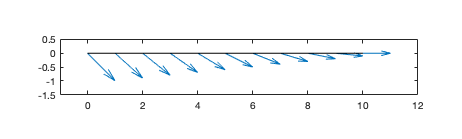
\includegraphics[scale=0.5]{img/C16vectorline.png}
\end{multicols}

Interpreting the output as a position, $t\mapsto \left\langle1,-1+\frac{t}{10}\right\rangle$ assigns a point in $2$-space to each value of $t$.  This function is illustrated below, where I have plotted the points $\left(1,-1+\frac{t}{10}\right)$ for eleven values of $t$.

\begin{multicols}{2}
\begin{lstlisting}
tval = 0:10;
plot(1+0*tval,-1+tval/10,'-*')
axis equal
\end{lstlisting}
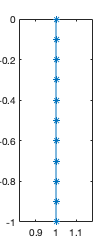
\includegraphics[scale=0.6]{img/C16curve.png}
\end{multicols}

\noindent\textbf{Parameterizing a circle}. 

In $\mathbb{R}^2$, the curve $x^2+y^2 = 1$ can be parameterized as $x(t) = \cos t, y(t) = \sin t,$ $0\leq t \leq 2\pi.$



% Parameterize a piece of a circle.  In this case the quarter circle of radius $2$ traversed from $(2,0)$ to $(0,2)$. \emph{pollQ}

% \includegraphics{img/N22_c2.pdf} 

\begin{enumerate}
\itemsep5em
\item Write parametric equations for a circle of radius $5$.
\item Write parametric equations for a circle of radius $1$ centered about $(2,-3)$.
\item Write parametric equations to traverse the unit circle once in the clockwise direction.
\item Write parametric equations to traverse a quarter circle.
\item Write parametric equations so that it takes time $1$ to traverse the circle, instead of time $2\pi$.
\item Write parametric equations for the ellipse $x^2+(y/2)^2 = 1$.
\end{enumerate}


\noindent\textbf{Parameterizing line segments} \S 17.1 
\begin{tcolorbox}
\begin{itemize}
\itemsep0em
    \item \textbf{Line segments} can be parameterized by the three equations \[x = x_0 + a t, \quad y = y_0 + b t, \quad z = z_0 + c t, \quad t_0 \leq t \leq t_1. \]
    \item The vector $\mb v = a\mb i +b\mb j + c\mb k$ is parallel to the line parameterized by $\mb r(t) = (x_0+at)\mb i + (y_0 + bt)\mb j + (z_0 + ct)\mb k = \mb r_0 + t\mb v$ where $\mb r(0) = x_0\mb i + y_0\mb j + z_0\mb k$ is interpreted as a position.
    \item A section of the curve given by the graph of $y = f(x)$ in $\mathbb{R}^2$ can be parameterized by $x = t,$ $y = f(t)$, $a\leq t\leq b$, or $\mb r(t) = t\mb i + f(t)\mb j$, $a\leq t\leq b$.
\end{itemize}
\end{tcolorbox}



\noindent\textbf{Point at time zero}.  What point does the line $\mb r(t)=(3+t)\mb i + 2t\mb j+ (-4-t)\mb k$ pass through when $t=0$?

%\emph{pollQ}

\vspace{1cm}

\noindent\textbf{Vector parallel to line}.
Find a vector aligned parallel to the line $\mb r(t)=(3+t)\mb i + 2t\mb j+ (-4-t)\mb k$.

\vspace{1cm}



\noindent\textbf{Piece of graph of function}

The curve below is a parabola with minimum at $(0,0)$.

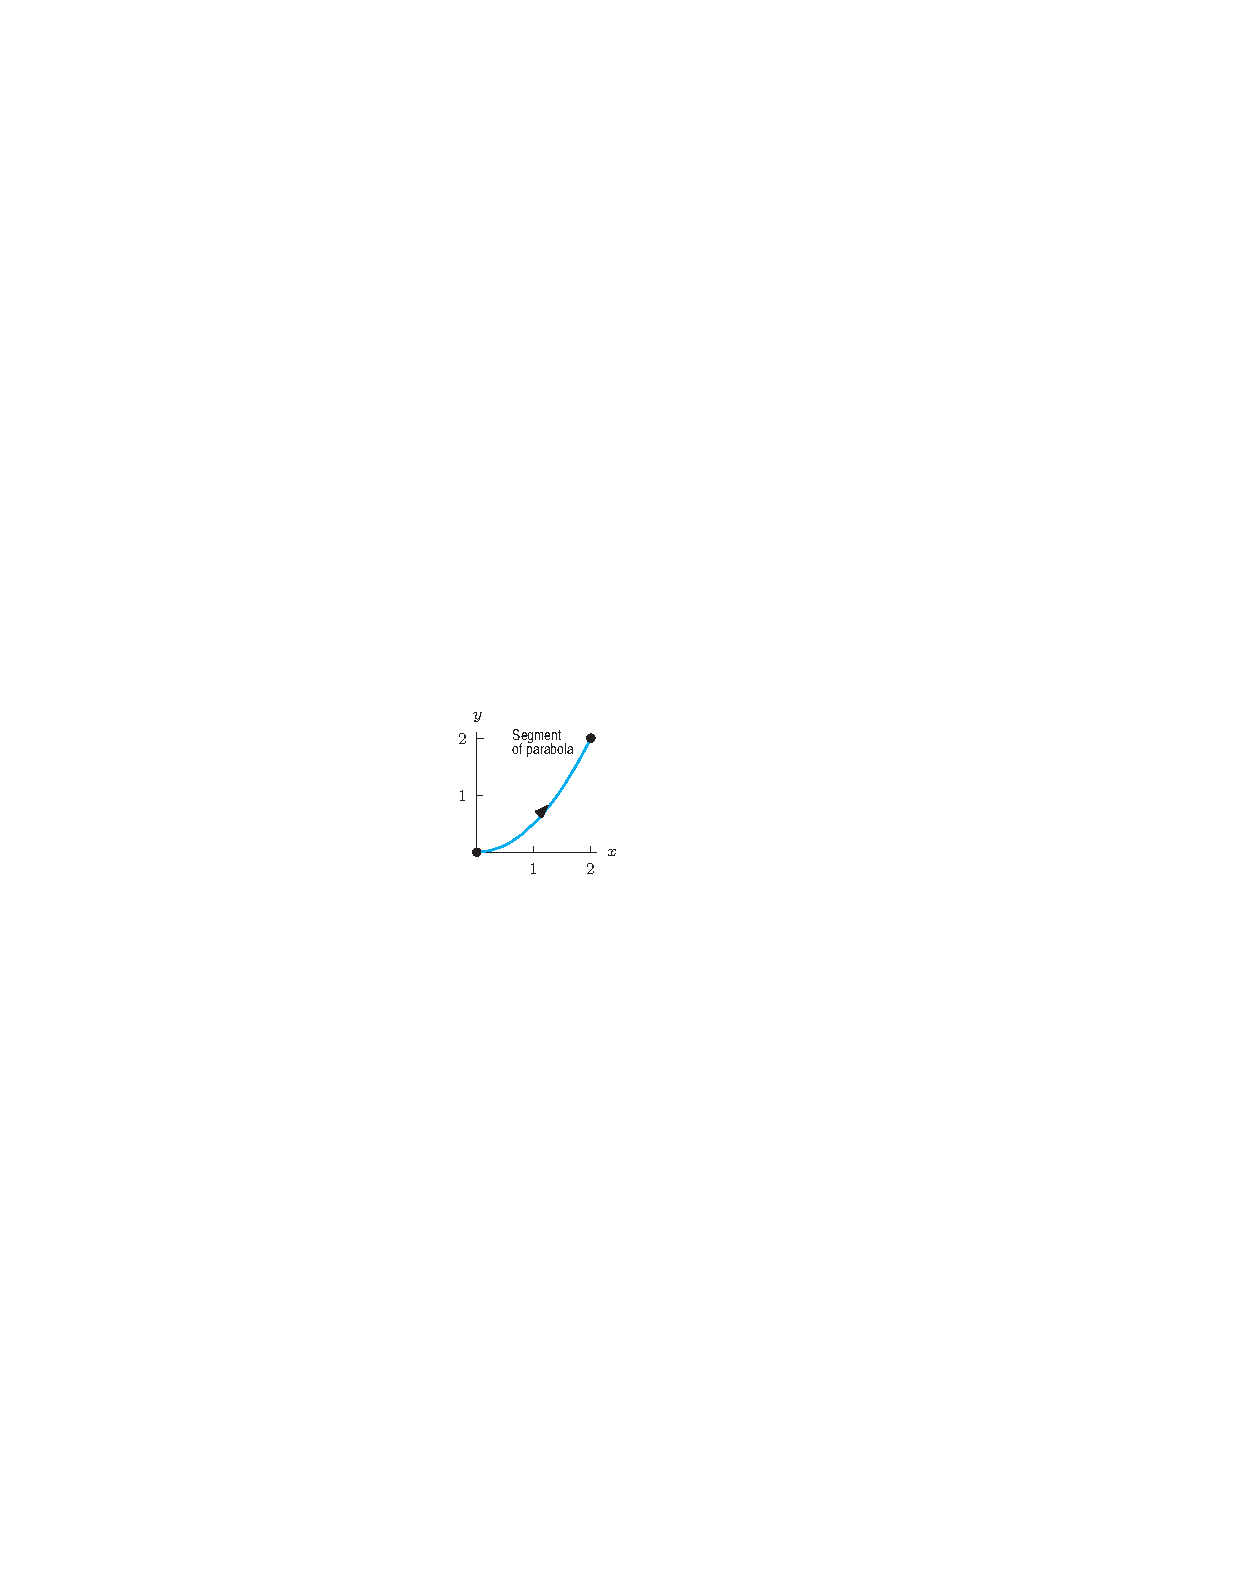
\includegraphics{img/N22_c4.pdf} 

Find a function such that the curve above is a piece of the function $y = f(x)$ and then create a parameterization of the curve. 

\vspace{2in}


\end{document}